\documentclass[usenames,dvipsnames,svgnames,table]{beamer}

\usetheme{AnnArbor}
\usepackage{lmodern}
\usepackage{amsmath}
\usepackage{enumitem}


\newcommand{\CMS}[1]{\textcolor{blue}{#1}}
\newcommand{\ATLAS}[1]{\textcolor{Green}{#1}}
\newcommand{\theory}[1]{\textcolor{red}{#1}}
\newcommand{\Sara}[1]{\textcolor{cyan}{#1}}
\newcommand{\me}[1]{\textbf{\CMS{#1}}}

\newcommand{\spin}[1]{\text{spin }#1}

\newenvironment{variableblock}[3]{
%http://tex.stackexchange.com/questions/33231/how-to-change-the-color-of-a-block-within-a-custom-beamer-sty-theme-file
  \setbeamercolor{block body}{#2}
  \setbeamercolor{block title}{#3}
  \begin{block}{#1}\end{block}}

\title[JHUGen and MELA]{Tools for the Higgs boson CP studies: \\ JHUGen and MELA}

\author[Heshy Roskes]{\CMS{I. Anderson}, \Sara{S. Bolognesi}, \theory{F. Caola}, \ATLAS{Y. Gao}, \CMS{A. Gritsan}, \theory{Z. Guo}, \CMS{C. Martin}, \theory{K. Melnikov}, \me{H. Roskes}, \CMS{U. Sarica}, \theory{M. Schulze}, \CMS{N. Tran}, \CMS{A. Whitbeck}, \CMS{M. Xiao}, \CMS{C. You}, \theory{Y. Zhou}
\texorpdfstring{\\ \leavevmode
\\
\ATLAS{ATLAS}, \CMS{CMS}, \theory{theory}, \Sara{where is Sara?}}{}}

\date{August 4, 2015}

%\author{I. Anderson, S. Bolognesi, F. Caola, Y. Gao, A. Gritsan, C. Martin, Z. Guo, K. Melnikov, {H. Roskes}, U. Sarica, M. Schulze, N. Tran, A. Whitbeck, M. Xiao, C. You, Y. Zhou}



\begin{document}

\begin{frame}
\titlepage
\end{frame}

\begin{frame}{Framework}

\begin{itemize}
\small
\item JHUGen
\begin{itemize}
\item Event generation
\end{itemize}
\item JHUGenMELA
\begin{itemize}
\item Discriminants for anomalous coupling fits and background suppression
\item Reweighting
\end{itemize}
\item AnalyticMELA
\begin{itemize}
\item Discriminants for anomalous coupling fits and background suppression
\item Validation
\end{itemize}
\end{itemize}

\end{frame}


\begin{frame}{JHU Generator}
\begin{itemize}
\item $gg\to\spin{0}$
\item $q\bar{q}\to\spin{1}$
\item $gg/q\bar{q}\to\spin{2}$
\end{itemize}
%\leavevmode \\
\begin{itemize}
\item
\begin{itemize}[label={$\to$}]
\item $ZZ^*+Z\gamma^*+\gamma^*\gamma^*\to \text{leptons+jets}$
\item $W^+W^-\to \text{leptons+jets}$
\item $Z\gamma$, $\gamma\gamma$
\end{itemize}
\end{itemize}
\end{frame}

\begin{frame}{JHU Generator---more Higgs production mechanisms}
\begin{itemize}
\item $gg/gq\to\spin{0}+\text{jet}$
\item $gg/gq/q\bar{q}\to\spin{0}+2\text{ jets}$ (QCD)
\item $q\bar{q}\to\spin{0}+2\text{ jets}$ (VBF)
\item $q\bar{q}\to V^*\to V+\spin{0}$ (VH)
\item $gg/q\bar{q}\to t\bar{t}H$, with $t\to Wb \to l\nu b/q\bar{q}^\prime b$
\item
\item
\item Ability to read input LHE files from other generators
\end{itemize}
\end{frame}

\begin{frame}{Parameterization}
\begin{itemize}
%\item Most general parameterization of anomalous couplings:
\item \small
$
A(HVV) \sim
$
\begin{itemize}
\item
$
\left[ a_{1}
+ \textcolor{Green}{\frac{q_{V_1}^2 +  q_{V_2}^{2}}{\left(\Lambda_{1} \right)^{2}}}
+ \textcolor{magenta}{\frac{(q_{V_1} + q_{V_2})^{2}}{\left(\Lambda_{Q} \right)^{2}}}
\right]
m_{V_1}^2 \epsilon_{V_1}^* \epsilon_{V_2}^*
+ \textcolor{red}{a_{2}  f_{\mu \nu}^{*(1)}f^{*(2),\mu\nu}}
+ \textcolor{blue}{a_{3}   f^{*(1)}_{\mu \nu} {\tilde f}^{*(2)\mu\nu}}
$
\end{itemize}
%\normalsize Lagrangian (equivalent)
\tiny
\item
$
 {L}(HVV) \sim
$
\begin{itemize}
\item
$
a^{ZZ}_{1}\frac{m_{Z}^2}{2} H Z^{\mu}Z_{\mu}
- \textcolor{Green}{\frac{1}{\left(\Lambda^{ZZ}_{1}\right)^{2}} m_{Z}^2 H  Z^{\mu} \Box Z_{\mu}}
- \textcolor{magenta}{\frac{1}{2\left(\Lambda^{ZZ}_{Q}\right)^{2}} m_{Z}^2 \Box H  Z^{\mu} Z_{\mu}}
- \textcolor{red}{\frac{1}{2}a^{ZZ}_{2} H  Z^{\mu\nu}Z_{\mu\nu}}
- \textcolor{blue}{\frac{1}{2}a^{ZZ}_{3} H  Z^{\mu\nu}{\tilde Z}_{\mu\nu}}
$
\item
$
+ a_{1}^{WW}{m_{W}^2} H W^{+\mu} W^{-}_{\mu}
- \textcolor{Green}{\frac{1}{\left(\Lambda_{1}^{WW}\right)^{2}} m_{W}^2 H
  \left(  W^{-}_{\mu} \Box W^{+\mu} + W^{+}_{\mu} \Box W^{-\mu} \right)}
$
\begin{itemize}
\item
$
- \textcolor{magenta}{\frac{1}{\left(\Lambda_{Q}\right)^{2}} m_{W}^2 \Box H  W^{+\mu} W^{-}_{\mu}}
- \textcolor{red}{a_{2}^{WW} H W^{+\mu\nu}W^{-}_{\mu\nu}}
- \textcolor{blue}{a_{3}^{WW} H W^{+\mu\nu}{\tilde W}^{-}_{\mu\nu}}
$
\end{itemize}
\item
$
+ \textcolor{Green}{\frac{1}{\left(\Lambda_{1}^{Z\gamma} \right)^{2}} m_{Z}^2 H  Z_\mu \partial_\nu F^{\mu\nu}}
- \textcolor{red}{a_{2}^{Z\gamma} H F^{\mu\nu} Z_{\mu\nu}}
- \textcolor{blue}{a_{3}^{Z\gamma} H  F^{\mu\nu}{\tilde Z}_{\mu\nu}}
$
\item
$
- \textcolor{red}{\frac{1}{2}a_{2}^{\gamma\gamma} H  F^{\mu\nu}F_{\mu\nu}}
- \textcolor{blue}{\frac{1}{2}a_{3}^{\gamma\gamma}H  F^{\mu\nu}{\tilde F}_{\mu\nu}}
$
\item
$
- \textcolor{red}{\frac{1}{2}a_{2}^{gg} H  G^{\mu\nu}_a G^a_{\mu\nu}}
- \textcolor{blue}{\frac{1}{2}a_{3}^{gg}H  G^{\mu\nu}_a{\tilde G}^a_{\mu\nu}}
$
\end{itemize}
\item \small Similar for spin 1 and spin 2
\item
\item Predictions are leading order QCD
\item Can read input LHE file and add anomalous Higgs decay
\begin{itemize}
\item POWHEG (NLO QCD) $gg\to H$ $\longrightarrow$ JHUGen anomalous decay
\end{itemize}
\end{itemize}
\end{frame}

\begin{frame}{JHUGen in action}{
%twiki: https://twiki.cern.ch/twiki/bin/view/CMSPublic/Hig14018PaperTwiki
Generation, reweighting, discriminants \hfill [CMS-HIG-14-018] arXiv:1411.3441
}
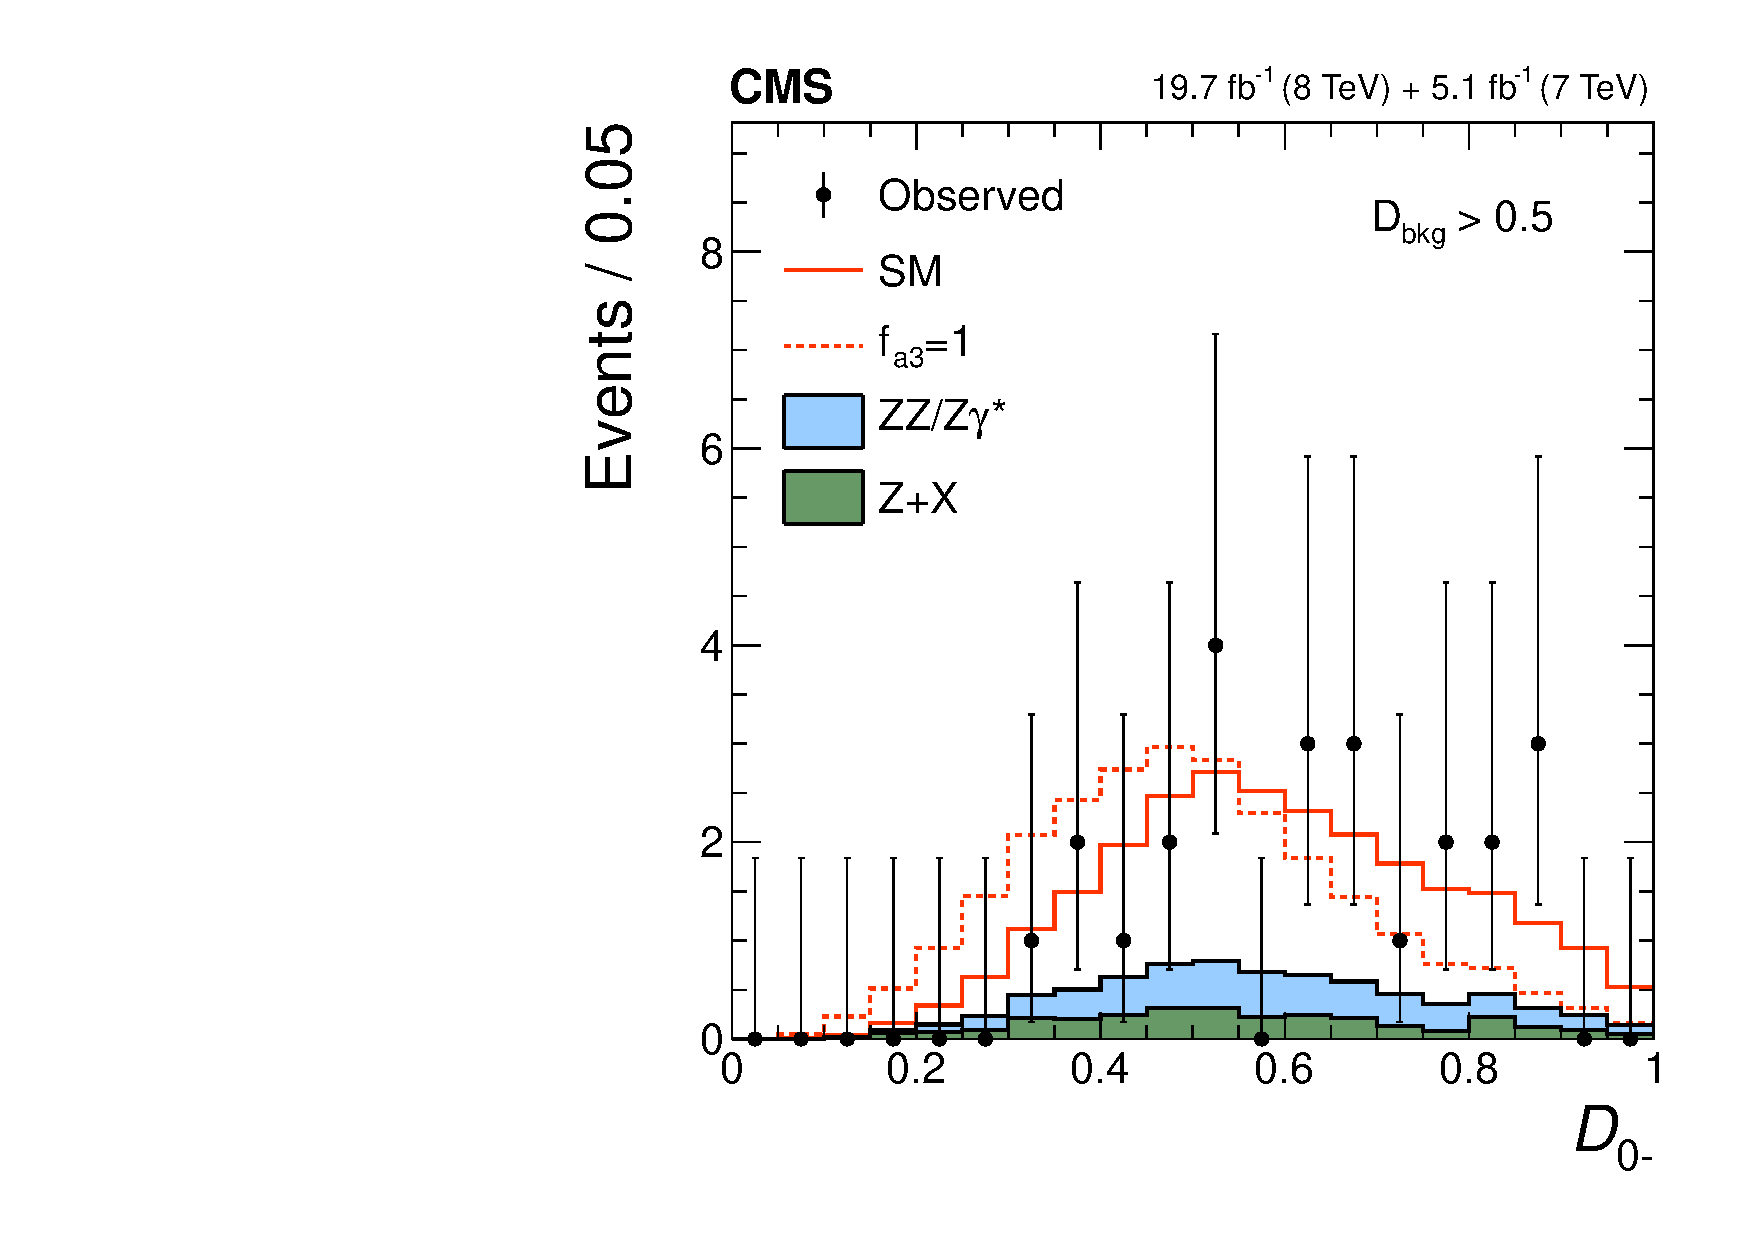
\includegraphics[width=0.25\textwidth]{d0minus}
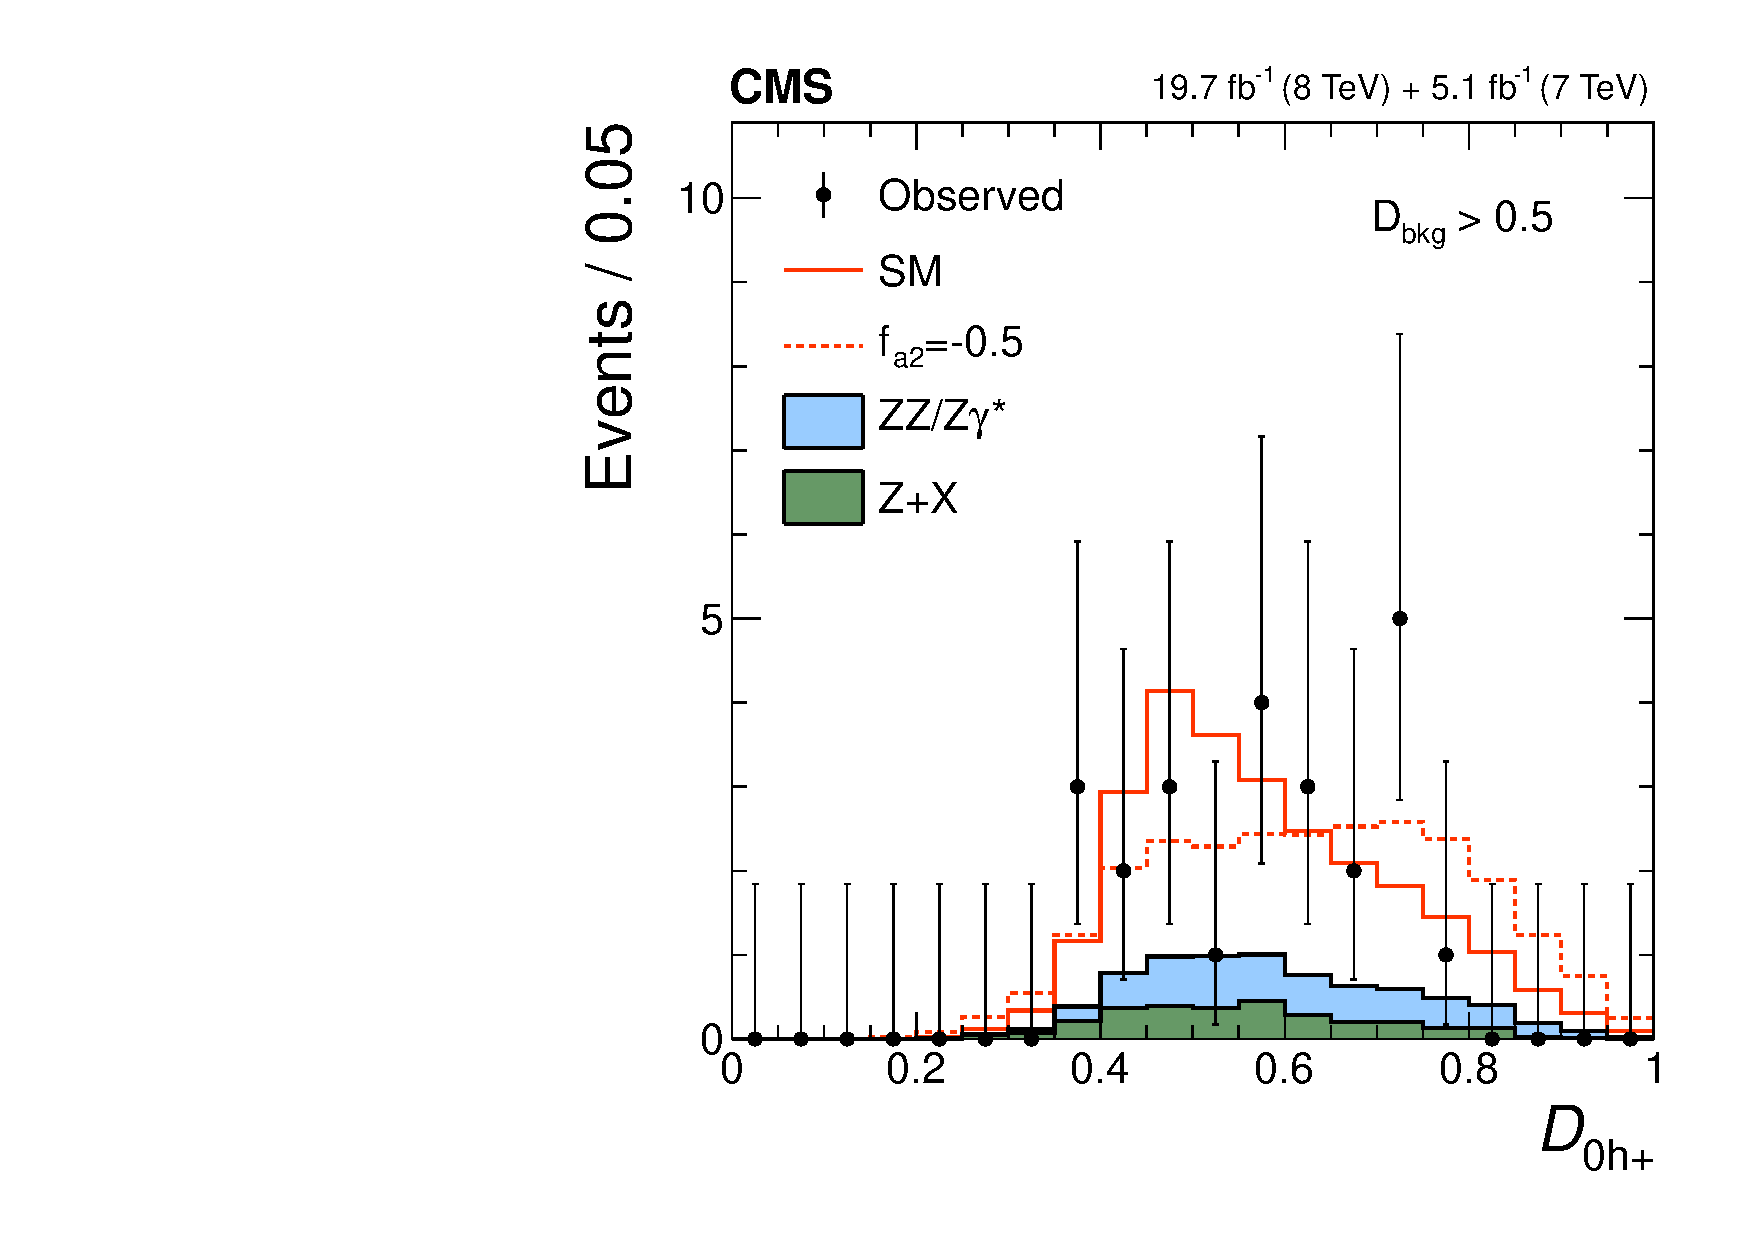
\includegraphics[width=0.25\textwidth]{d0hplus}
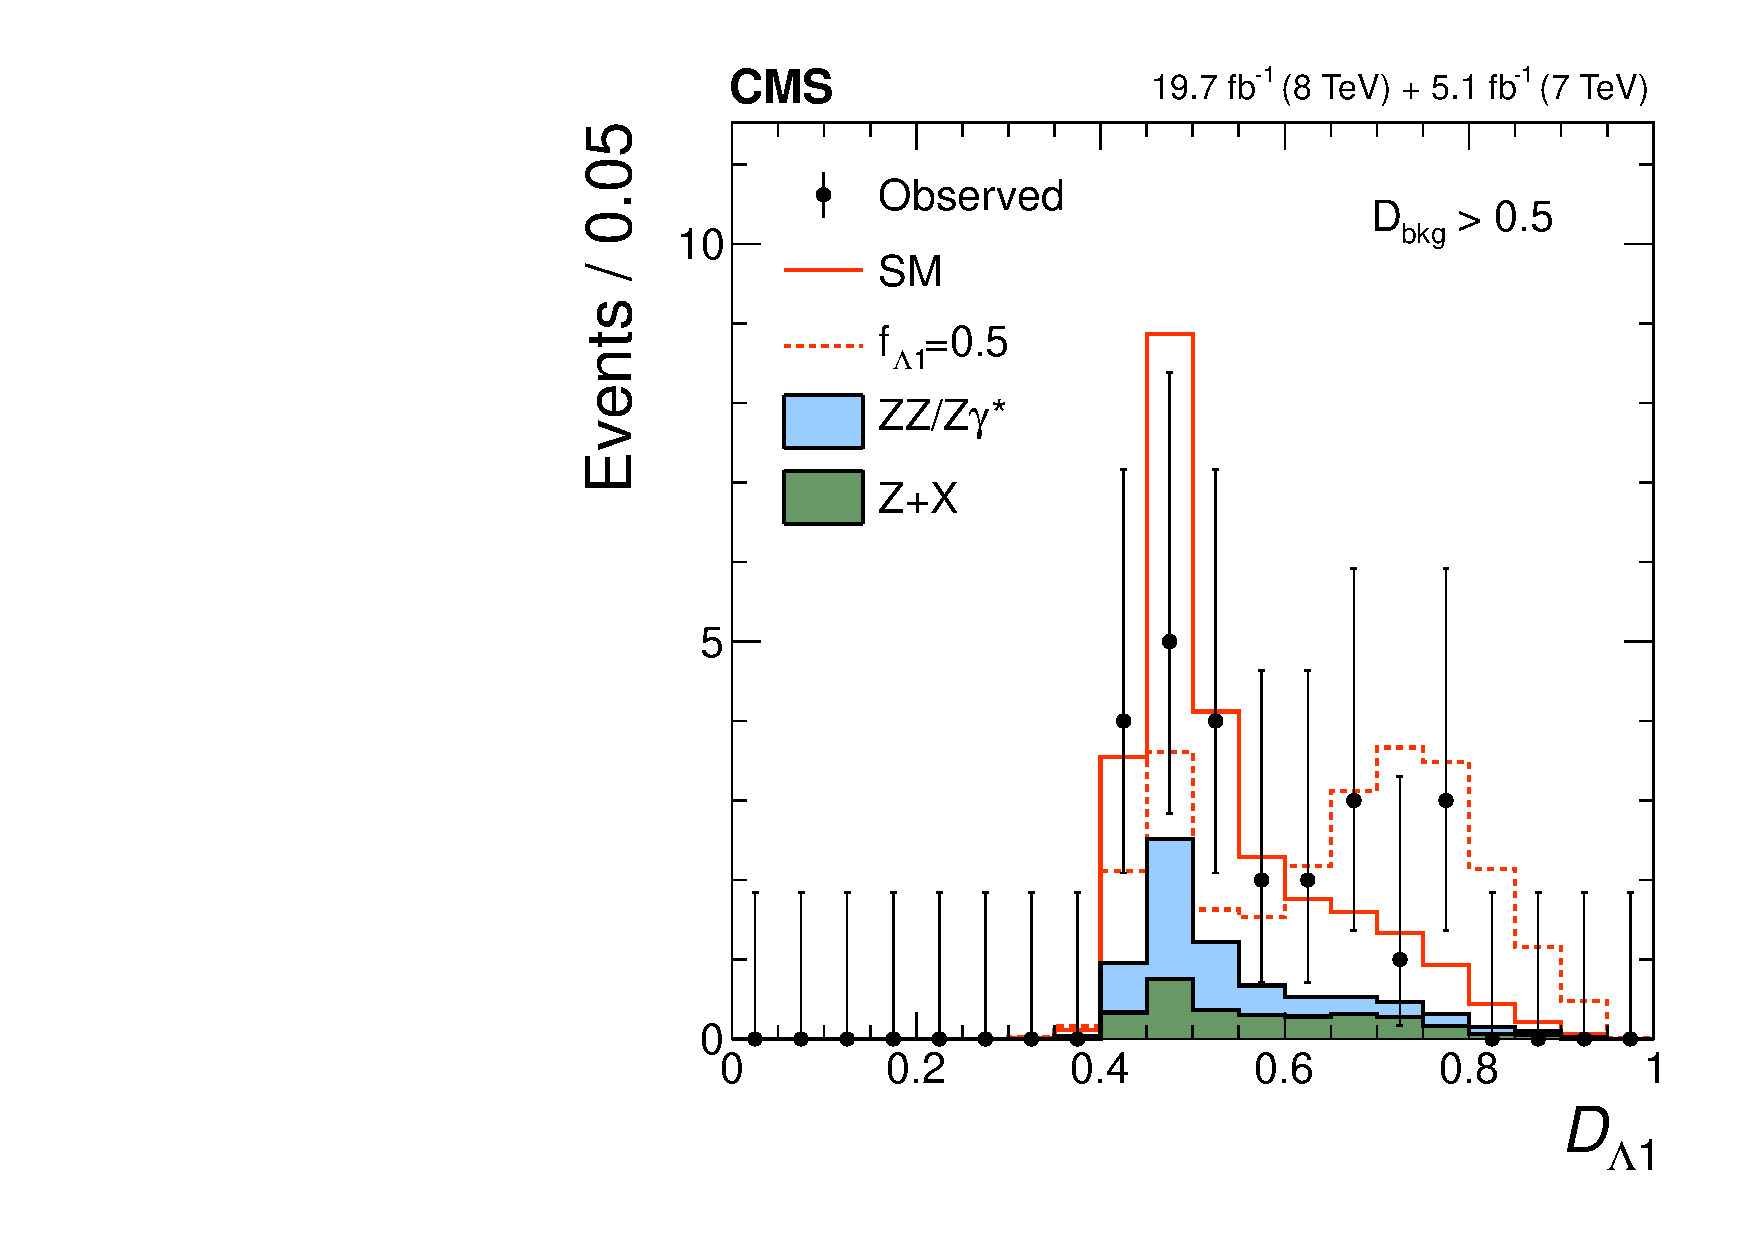
\includegraphics[width=0.25\textwidth]{dlambda1}
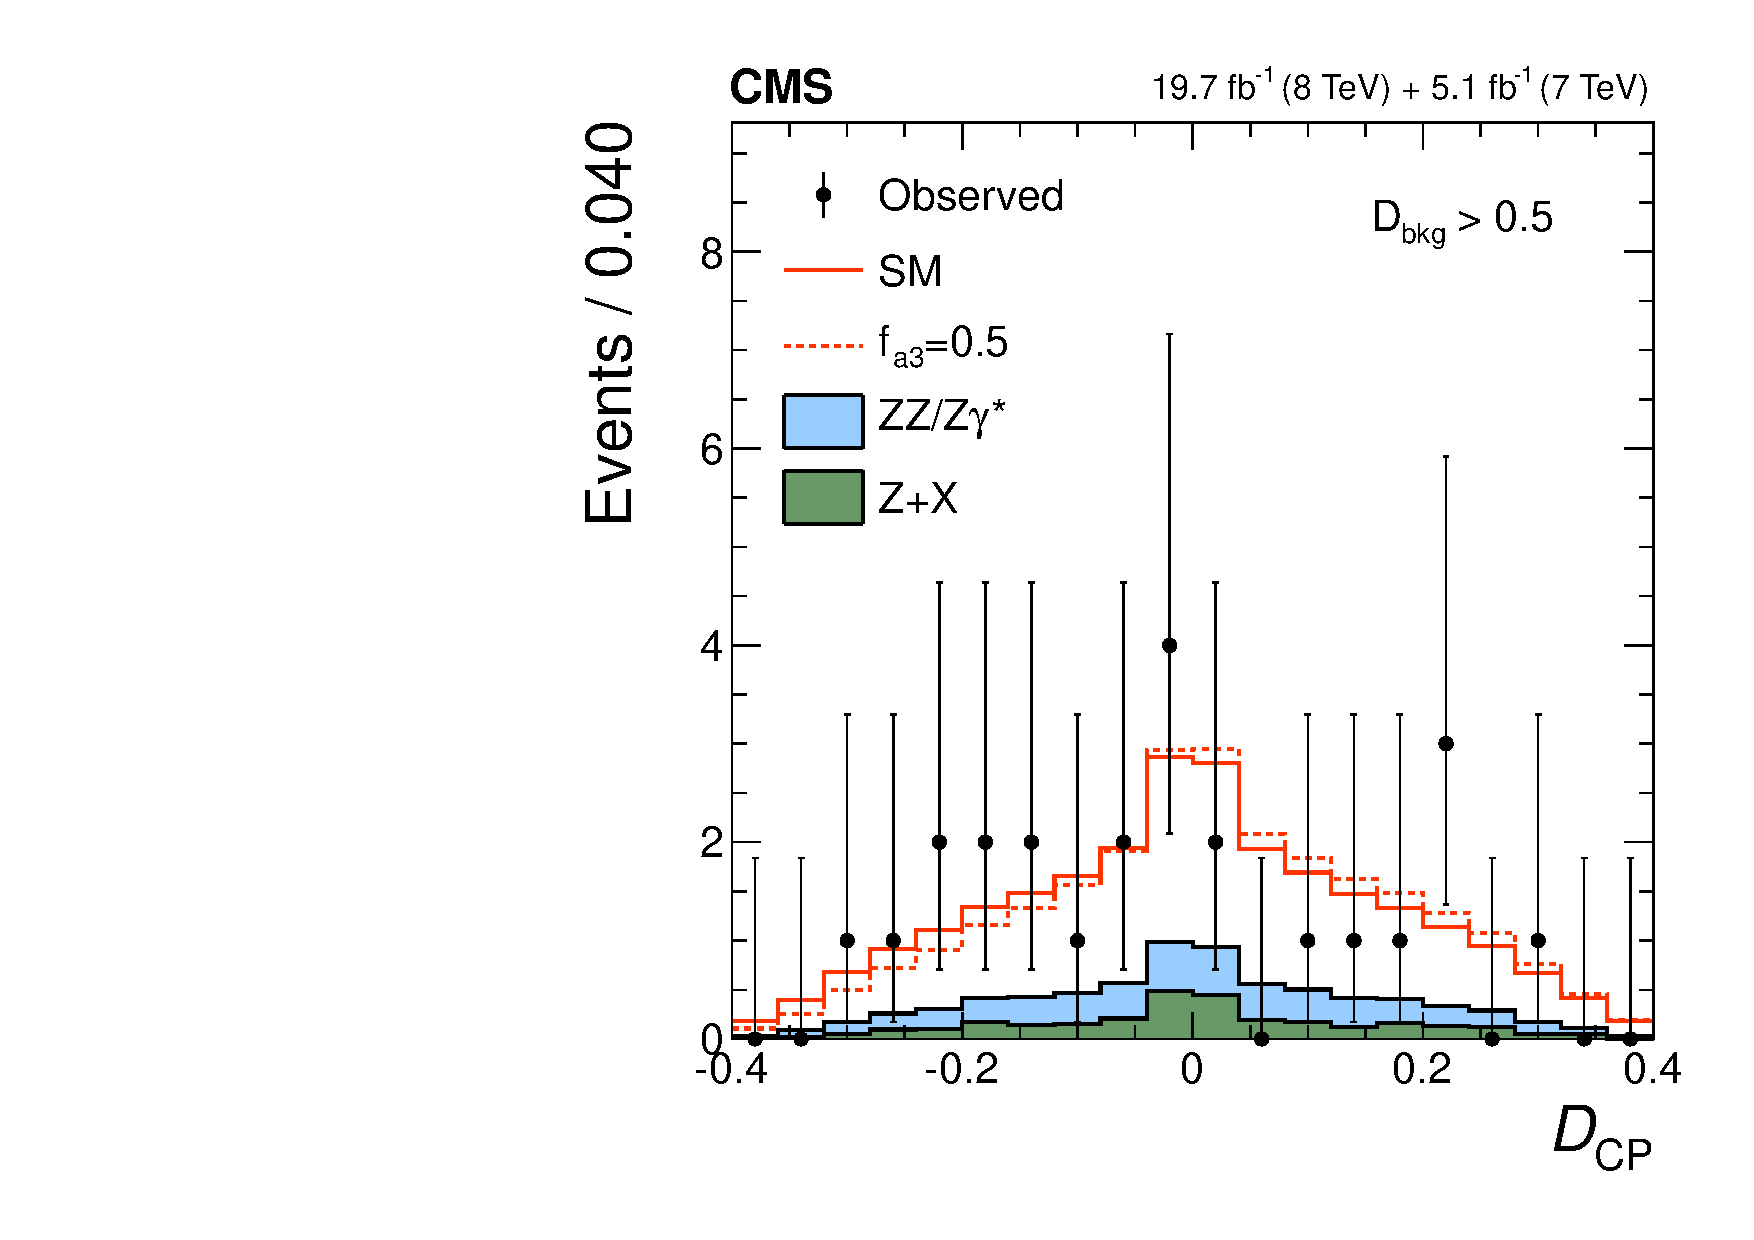
\includegraphics[width=0.25\textwidth]{dcp}
\\
\begin{columns}
\begin{column}{0.6\textwidth}
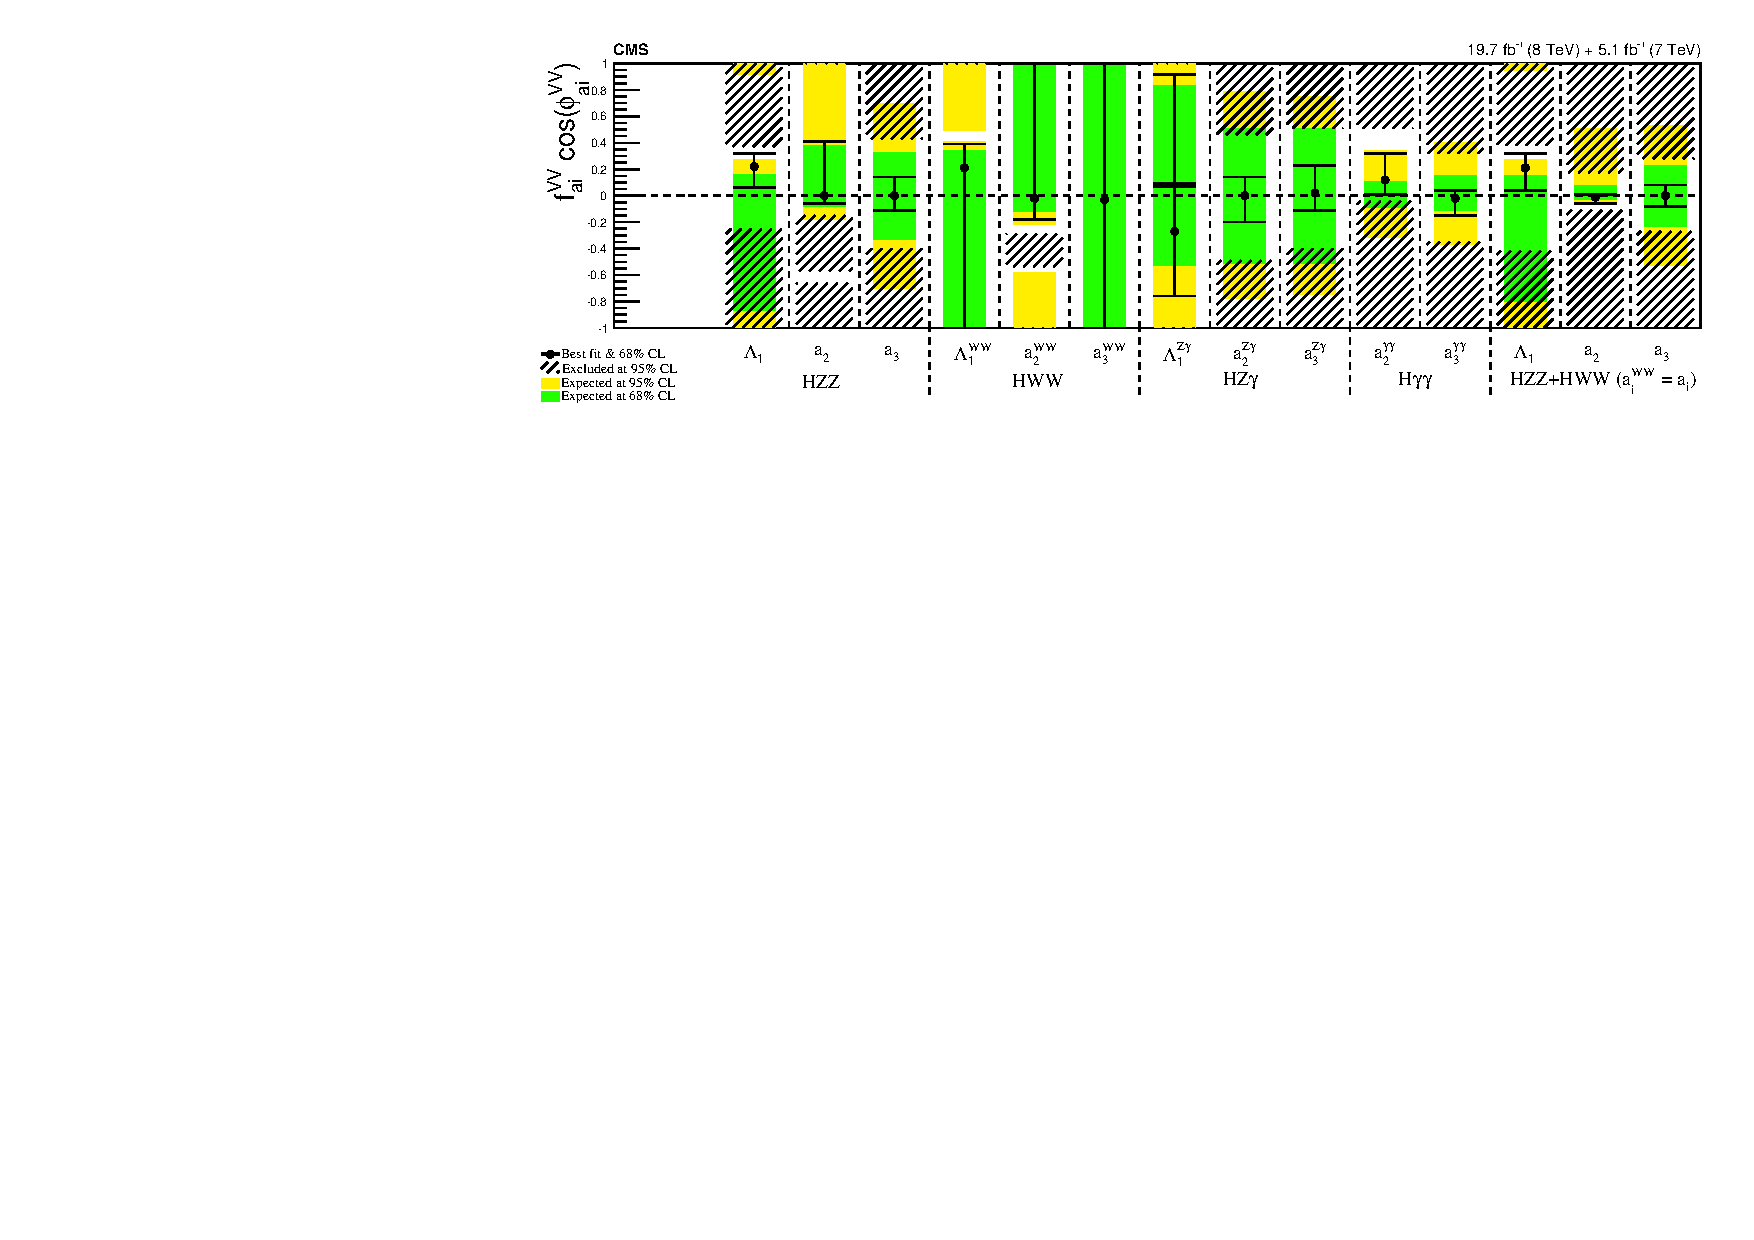
\includegraphics[width=\textwidth]{summary_a2a3lambda1}
\end{column}
\begin{column}{0.4\textwidth}
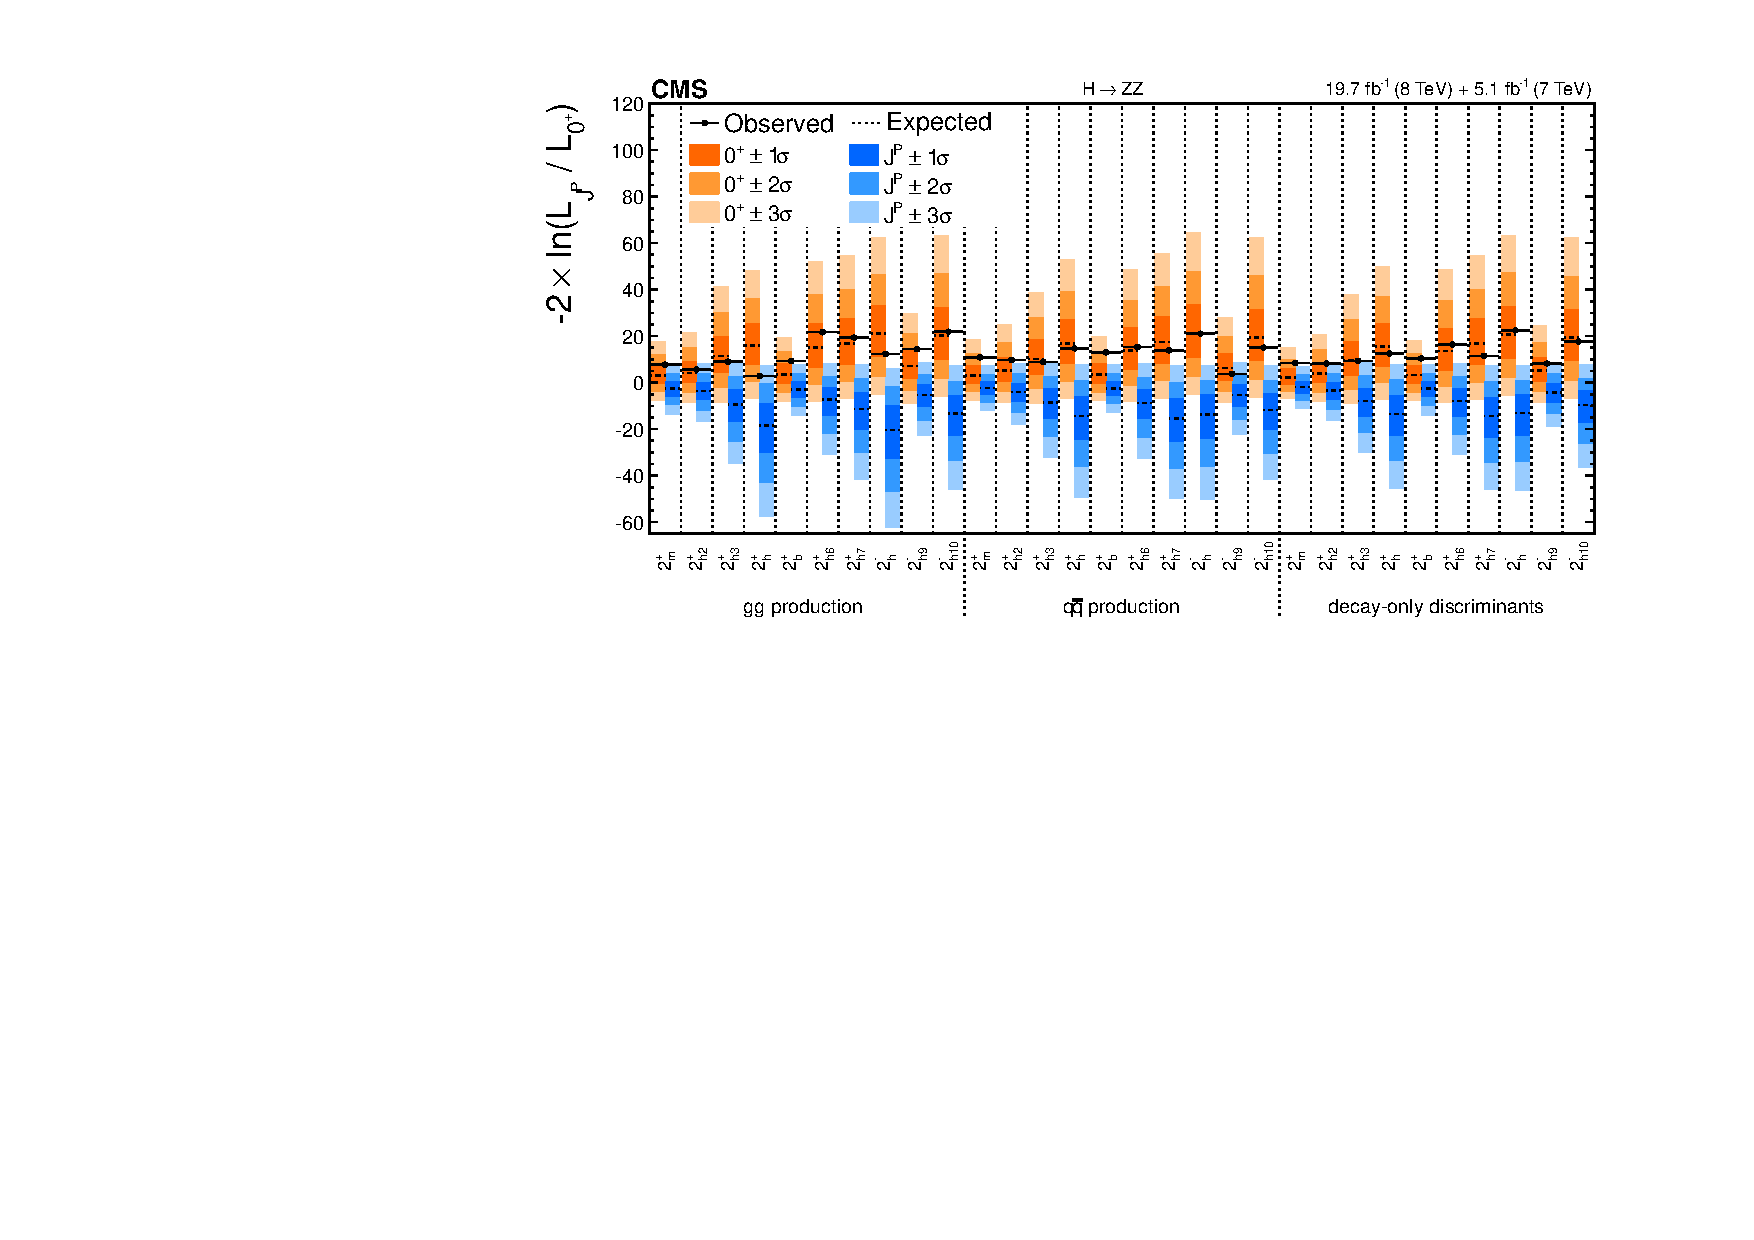
\includegraphics[width=\textwidth]{JP_SummaryPlot}
\end{column}
\end{columns}
\end{frame}



\end{document}
